\documentclass[12pt,a4paper]{article}

\usepackage[utf8]{inputenc}
\usepackage[T1]{fontenc}
\usepackage[french]{babel}
\usepackage{geometry}
\usepackage{hyperref}
\usepackage{listings}
\usepackage{xcolor}
\usepackage{titlesec}
\usepackage{enumitem}
\usepackage{fancyhdr}
\usepackage{graphicx}
\usepackage{float}
\usepackage{dirtree}
\usepackage{fancyvrb}
\usepackage{amsmath}
\usepackage{microtype}
\usepackage{parskip}

\geometry{margin=2.5cm}

\definecolor{codegray}{rgb}{0.95,0.95,0.95}
\definecolor{codeblue}{rgb}{0.13,0.29,0.53}
\definecolor{codecomment}{rgb}{0.4,0.4,0.4}

\lstdefinestyle{code3addr}{
    backgroundcolor=\color{codegray},
    basicstyle=\ttfamily\small,
    keywordstyle=\color{codeblue}\bfseries,
    commentstyle=\color{codecomment}\itshape,
    frame=single,
    framerule=0pt,
    rulecolor=\color{codegray},
    breaklines=true,
    captionpos=b,
    xleftmargin=1em,
    xrightmargin=1em,
    aboveskip=0.5em,
    belowskip=0.5em,
}

\lstset{style=code3addr,
    extendedchars=true,
    inputencoding=utf8,
    literate=
        {é}{{\'e}}1 {è}{{\`e}}1 {ê}{{\^e}}1 {ë}{{\"e}}1
        {à}{{\`a}}1 {â}{{\^a}}1 {ä}{{\"a}}1
        {ù}{{\`u}}1 {û}{{\^u}}1 {ü}{{\"u}}1
        {î}{{\^i}}1 {ï}{{\"i}}1
        {ô}{{\^o}}1 {ö}{{\"o}}1
        {ç}{{\c{c}}}1
        {É}{{\'E}}1 {È}{{\`E}}1 {Ê}{{\^E}}1
        {À}{{\`A}}1 {Â}{{\^A}}1
        {Î}{{\^I}}1 {Ô}{{\^O}}1 {Ù}{{\`U}}1 {Û}{{\^U}}1
        {«}{{\guillemotleft}}1 {»}{{\guillemotright}}1,
}

\pagestyle{fancy}
\fancyhf{}
\rhead{\small STRUCIT --- Mini Compilateur C}
\lhead{\small Mezrhab - Tripnaux-Moreau}
\rfoot{\thepage}
\renewcommand{\headrulewidth}{0.4pt}

\titleformat{\section}{\large\bfseries}{}{0em}{}
\titleformat{\subsection}{\normalsize\bfseries}{\thesubsection.}{0.5em}{}

\setlist[itemize,1]{label=--}
\setlist[itemize,2]{label=--}

\setlength{\parskip}{0.5em}

\begin{document}

\begin{titlepage}
  \centering
  \vspace*{3cm}
  {\Huge\bfseries Rapport d'Implémentation\par}
  \vspace{0.5cm}
  {\LARGE STRUCIT : Mini Compilateur C\par}
  \vspace{2cm}
  {\large Licence 3 Informatique\par}
  {\large Module de Compilation\par}
  \vspace{0.5cm}
  {\large Université Côte d'Azur\par}
  {\large Pr Sid Touati\par}
  \vspace{2cm}
  {\large\bfseries Bouchra Mezrhab \\ Mathéo Tripnaux-Moreau\par}
  \vfill
  {\normalsize\today\par}
\end{titlepage}

\tableofcontents
\newpage

\section{Introduction au projet}

Pour appréhender correctement le processus de compilation, il nous est demandé de programmer un mini-compilateur en C pour STRUCIT-frontend, un sous-ensemble du langage C, vers STRUCIT-backend, un dialecte C trois-adresses. Ces dernières semaines, nous avons produit un code effectif et adressé la totalité des points mentionnés par l'énoncé. Malgré plusieurs écueils, le projet dans sa version finale répond parfaitement à nos attentes.

Le compilateur est articulé en deux binaires indépendants : \texttt{structit} (frontend) et \texttt{structit\_backend} (backend). Le frontend lit un fichier STRUCIT-frontend et produit un fichier de code trois-adresses. Le backend lit ce fichier et valide sa conformité syntaxique. Le tout est automatisé par un Makefile et une pipeline CI sous GitHub Actions.

\vspace{2cm}

\begin{figure}[H]
  \centering
  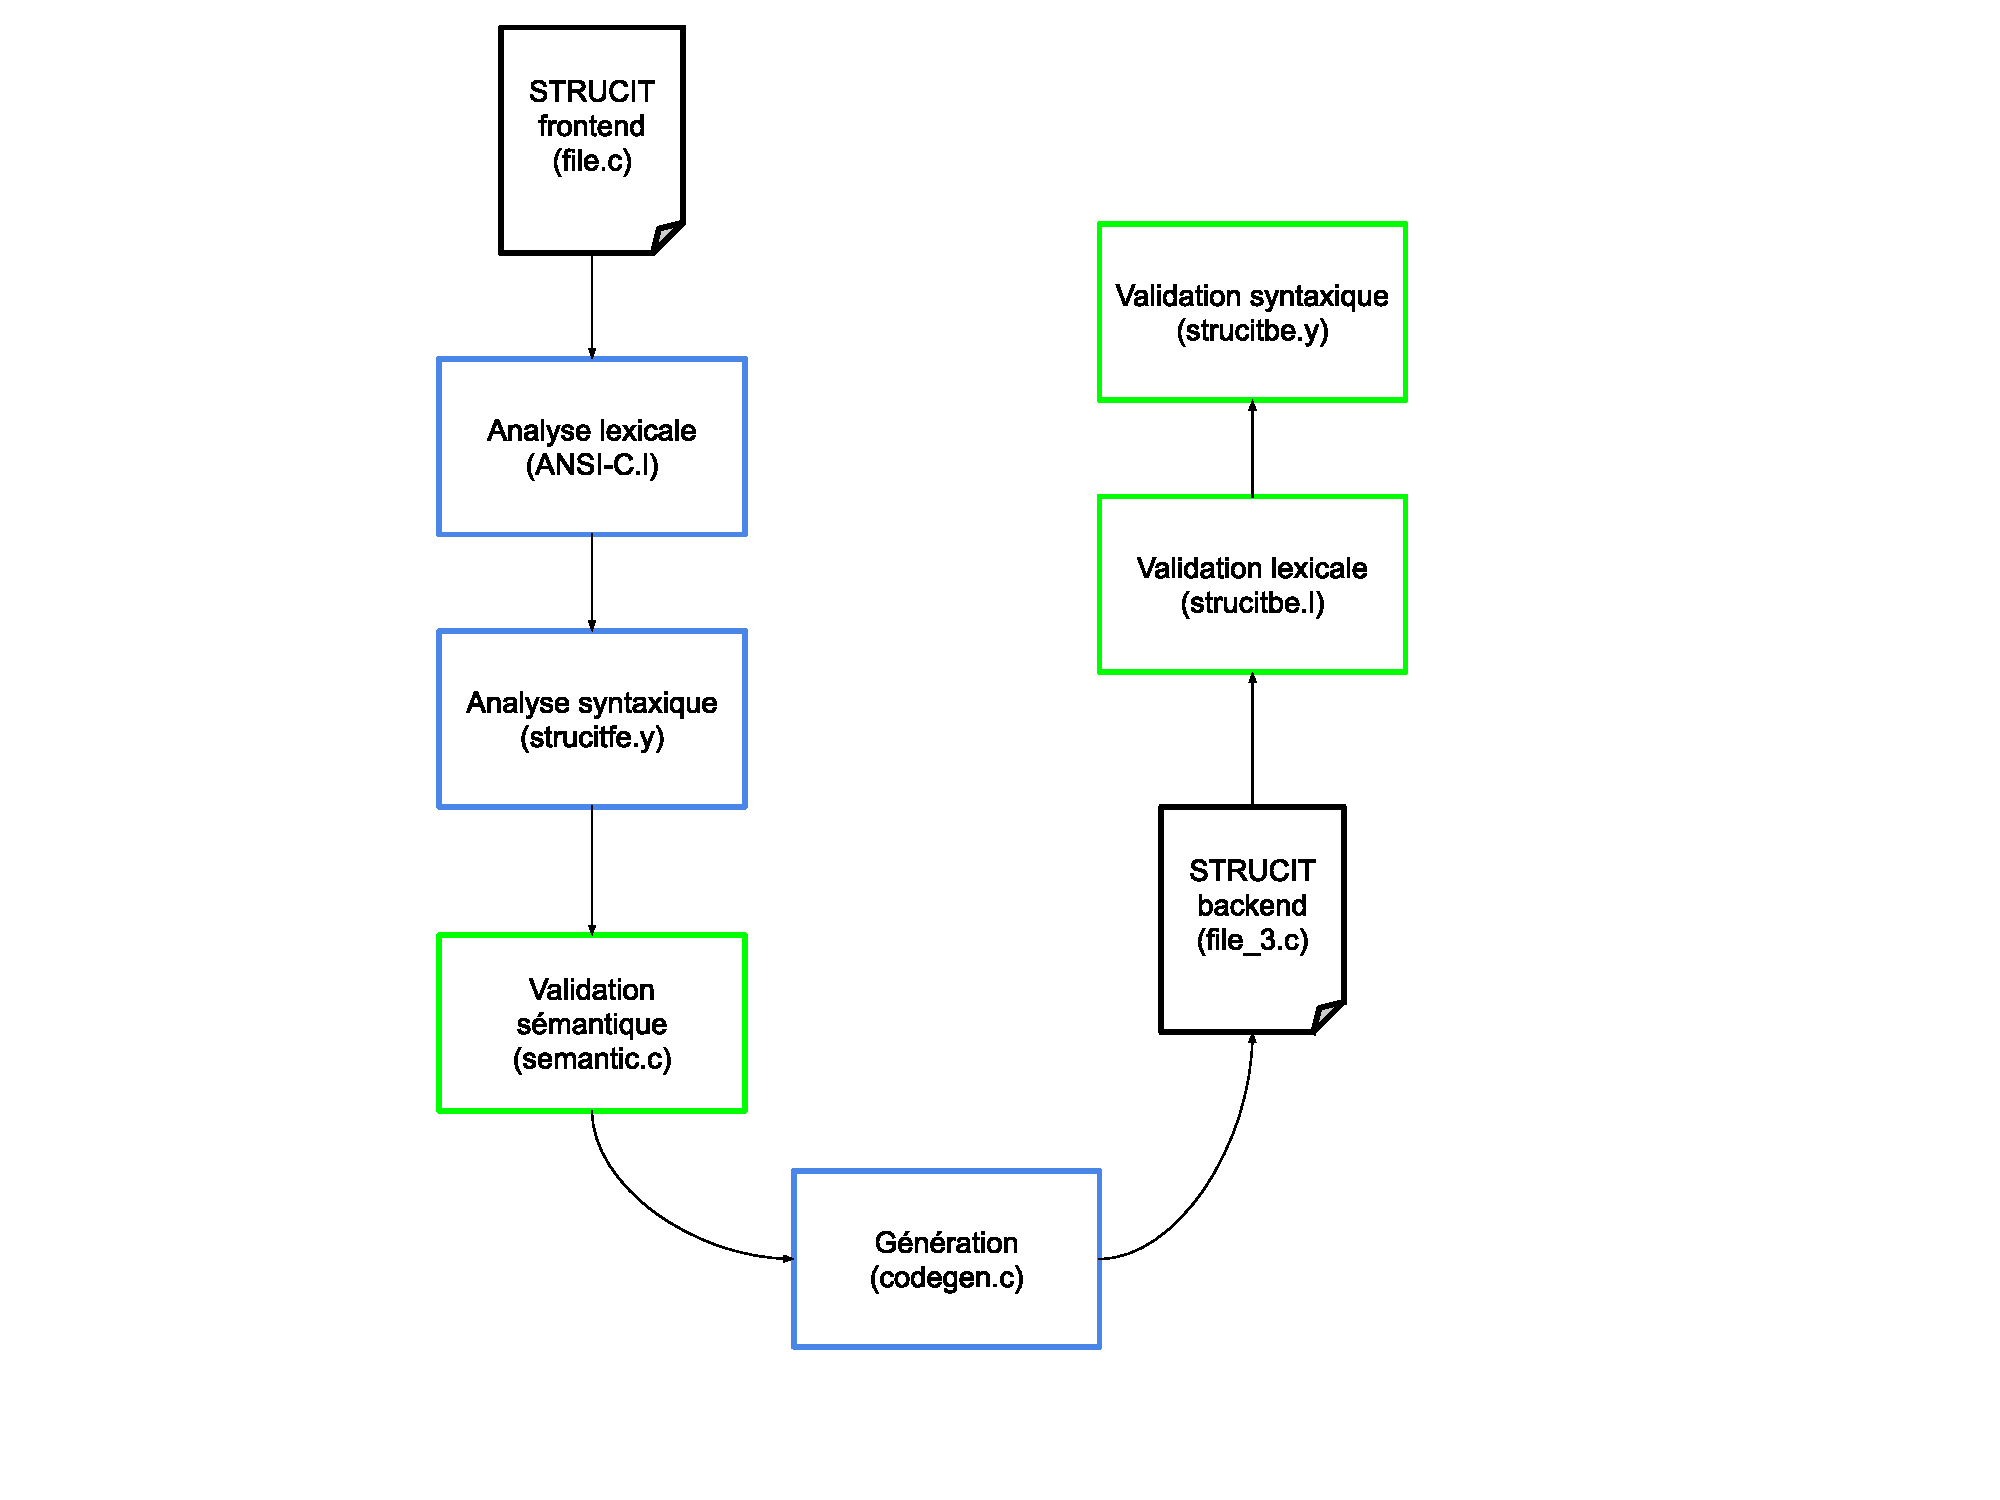
\includegraphics[width=\linewidth]{schema.pdf}
  \caption{Vue d'ensemble de la chaîne de génération et de validation}
  \label{fig:pipeline}
\end{figure}

\section{Architecture générale}

\subsection{Organisation des fichiers}

\begin{figure}[H]
\centering
\begin{BVerbatim}
strucit/
`-- source/
    |-- backend/
    |   |-- strucitbe.l
    |   `-- strucitbe.y
    `-- frontend/
        |-- ANSI-C.l
        |-- strucitfe.y
        |-- semantic.c
        |-- codegen.c
        |-- ast.c
        `-- symbol.c
\end{BVerbatim}
\caption{Arborescence des sources}
\end{figure}

\subsection{Pipeline de compilation}

La chaîne de traitement complète est la suivante :

\begin{enumerate}
  \item \textbf{Analyse lexicale} (\texttt{ANSI-C.l}) : découpage du source en tokens (mots-clés, identifiants, constantes, opérateurs).
  \item \textbf{Analyse syntaxique} (\texttt{strucitfe.y}) : construction de l'AST nœud par nœud selon la grammaire STRUCIT.
  \item \textbf{Analyse sémantique} (\texttt{semantic.c}) : vérification des déclarations et des arités d'appel.
  \item \textbf{Génération de code} (\texttt{codegen.c}) : parcours récursif de l'AST vers le dialecte trois-adresses.
  \item \textbf{Validation backend} (\texttt{strucitbe.l} + \texttt{strucitbe.y}) : vérification syntaxique du fichier généré.
\end{enumerate}

\section{Structures de données utilisées}

\subsection{Arbre Syntaxique Abstrait (AST)}

L'analyse lexico-syntaxique construit progressivement un arbre représentant le fichier STRUCIT-frontend dans son entièreté. Chaque construction est un nœud dont les enfants sont les sous-parties qui la composent. L'arité d'un nœud n'est pas fixe : un \texttt{AST\_PARAM\_LIST} peut avoir autant d'enfants que de paramètres, alors qu'un \texttt{AST\_OP} en a exactement deux. Les feuilles (identifiants et constantes entières) sont créées par le lexer ; les nœuds internes par les actions Yacc. Les mots clés ne deviennent pas des nœuds, mais déterminent la nature du nœud parent.

Chaque nœud porte un champ \texttt{line} (numéro de ligne source), propagé depuis le lexer via \texttt{yylineno}, ce qui permet d'afficher des messages d'erreur précis. Le champ \texttt{id} stocke indifféremment un nom d'identifiant ou un symbole d'opérateur (\texttt{"+"}, \texttt{"->"}, …). Le champ \texttt{size} est utilisé pour les calculs de \texttt{sizeof} et les tailles de structures.

\medskip
\textbf{Choix de représentation.} Les enfants d'un nœud sont stockés dans un tableau alloué dynamiquement (\texttt{realloc} à chaque \texttt{ast\_add\_child}). Deux alternatives ont été écartées. Un arbre binaire strict (fils gauche / fils droit) forçait à chaîner les instructions d'un bloc vers la droite, déséquilibrant l'arbre et risquant un débordement de pile sur les longs programmes. Un chaînage horizontal par pointeur \texttt{next} (liste d'instructions à plat) aurait simplifié le parcours séquentiel mais compliqué les nœuds qui mélangent enfants structuraux et instructions (un \texttt{AST\_FOR} a quatre sous-arbres de natures différentes). Le tableau dynamique unifie les deux cas sans distinction.

\subsection{Table de symboles}

Pour chaque identifiant (variable ou fonction) rencontré, son type et un \texttt{struct\_name} (le nom de la structure pointée) sont conservés et propagés si besoin. La table nous sert à :
\begin{itemize}
  \item déterminer si un temporaire doit être de type \texttt{int} ou \texttt{void*} ;
  \item calculer l'offset d'un champ dans une structure pour les accès via \texttt{->} ;
  \item déterminer le type de retour d'une fonction lors de la génération d'un appel ;
  \item vérifier le nombre d'arguments lors de l'analyse sémantique.
\end{itemize}

La table est organisée en deux niveaux : un scope global (\texttt{g\_global}) construit une fois pour le programme entier, et un scope local (\texttt{g\_local}) reconstruit à chaque définition de fonction.

\medskip
\textbf{Choix de représentation.} Nous avons retenu une arborescence de symboles (un nœud \texttt{Symbol} avec un tableau d'enfants) plutôt qu'une liste chaînée LIFO ou une table de hachage. La raison principale est que STRUCIT ne comporte pas de portées imbriquées à l'intérieur des fonctions : les seules portées sont globale et locale. Le masquage de variables entre blocs n'est donc pas un problème à gérer. Une liste LIFO aurait compliqué la recherche par nom de struct (nécessitant un parcours linéaire sans critère d'arrêt naturel), et une table de hachage aurait apporté une complexité d'implémentation sans gain notable sur des programmes de la taille attendue.

\subsection{Variables temporaires (registres)}

Un tableau de temporaires est généré, avec \texttt{g\_temp\_type} indiquant le type de chaque temporaire (\texttt{int} ou \texttt{void*}) et \texttt{g\_temp\_used} précisant si le registre est libre. On maintient aussi un compteur \texttt{g\_temp\_compteur}. Ce pool permet la réutilisation des temporaires libérés entre instructions (voir section~\ref{sec:sethi}).

\section{Organisation du travail}

Nous avons directement opté pour une collaboration asynchrone standard, via git et la plateforme GitHub, conjointement à une messagerie instantanée. Plusieurs rendez-vous en présentiel ont été organisés, notamment pour l'harmonisation des machines et la direction du projet. Les parties lexicale et syntaxique ont été réalisées petit à petit, en suivant une organisation stigmergique (charge de travail détaillée dans un document commun, chacun fait ce qu'il reste à faire dans l'ordre des priorités). Ensuite, il a été convenu que Mathéo implémenterait l'algorithme Sethi-Ullman. Cependant (détaillé à la section suivante), Bouchra a finalement participé à cette étape en y ajoutant la réutilisation des registres. Enfin, ce rapport ainsi que le support de soutenance sont rédigés conjointement via Overleaf, un éditeur \LaTeX{} en ligne permettant la collaboration en temps réel.

Concrètement, Mathéo a réécrit le parser frontend, mis en place l'architecture et le Makefile, intégré une pipeline de tests CI sous container Debian, ré-aligné plusieurs fois le projet sur la grammaire de l'énoncé, et pris en charge la correction des fuites mémoire (ownership de \texttt{g\_expr\_sname}, libération de \texttt{g\_local}, des tableaux de temporaires et des tables de symboles). Bouchra a développé la couche intermédiaire, incluant l'AST et l'analyse syntaxique backend. La génération de code a été co-écrite itérativement en intégralité, de même que l'analyse sémantique et que la table des symboles.

\section{Problèmes de fond rencontrés}

\subsection{Sethi-Ullman : ordre d'évaluation vs réutilisation de registres}
\label{sec:sethi}

L'algorithme Sethi-Ullman minimise le nombre de registres simultanément actifs en ordonnant l'évaluation des sous-arbres (lourd en premier). Dans un code trois adresses, on obtient un ordre d'instructions optimal. Mais la réutilisation des temporaires entre instructions relève de l'allocation de registres, ce qui est un problème distinct, qui s'est trouvé plus difficile à implémenter que l'algorithme en lui-même, principalement à cause du manque de ressources traitant ce cas précis.

Concrètement, l'algorithme de Sethi-Ullman calcule un entier par nœud de l'AST (fonction \texttt{su\_label}) représentant la profondeur de la sous-expression. La génération choisit ensuite d'évaluer en premier l'enfant de poids le plus élevé. La réutilisation est assurée par le pool \texttt{g\_temp\_used[]} : \texttt{liberer\_temp()} marque un temporaire comme libre, \texttt{creer\_temp()} le réattribue si son type correspond.

\subsection{Représentation des types : tout aplati en \texttt{int} / \texttt{void*}}

L'énoncé distingue \texttt{int}, \texttt{void}, pointeurs sur struct, pointeurs sur int, pointeurs sur fonctions. En backend, tous les pointeurs deviennent \texttt{void*}. Cette simplification est conforme à l'énoncé mais a pour conséquences la perte de l'information de type, donc les appels de fonctions via pointeur se font nécessairement sans cast (\texttt{void*} directement).

\subsection{\texttt{sizeof} : taille du pointeur ou de la structure pointée}

L'énoncé dit : \textit{« sizeof retourne la taille en octets de la structure pointée par la variable »}. En C standard, \texttt{sizeof(p)} pour un pointeur retourne 4 (taille du pointeur). Après avoir implémenté la sémantique C standard, nous nous sommes rendus compte que dans les exemples donnés, \texttt{sizeof(p)} avec \texttt{p} de type \texttt{struct liste *} génère 4 alors que la structure fait 8 octets. Les deux valeurs apparaissant dans les exemples de l'énoncé selon le contexte, nous avons choisi de suivre le standard C.

\subsection{Écarts entre \texttt{ANSI-C.l} fourni et la grammaire de l'énoncé}

Le fichier \texttt{ANSI-C.l} fourni est un squelette ANSI C complet qui contient des tokens absents de la grammaire STRUCIT-frontend : \texttt{<<}, \texttt{>>}, \texttt{++}, \texttt{--}. Tous sont à ignorer selon l'énoncé, mais les retourner depuis le lexer les rendait implicitement utilisables --- or les fichiers de test fournis par le professeur utilisent \texttt{<<} et \texttt{++}, tout en indiquant que tous les tests doivent passer. Après discussion, nous avons choisi de nous tenir strictement aux grammaires de l'énoncé : \texttt{<<}/\texttt{>>} sont supprimés des deux lexers et grammaires ; pour \texttt{++}/\texttt{--}, les règles de grammaire ont été retirées, le lexer retourne toujours le token mais le parser échoue immédiatement. Les tests concernés sont donc classés en erreurs attendues.

\subsection{Gestion mémoire : ownership ambigu de \texttt{g\_expr\_sname}}

La génération de code propage le nom de la structure courante via une variable globale \texttt{g\_expr\_sname} (\texttt{const char *}), mise à jour à chaque nœud d'expression. Cette variable peut pointer indifféremment vers un champ \texttt{struct\_name} appartenant à la table de symboles (mémoire non-propriétaire) ou vers une chaîne allouée localement. Cette ambiguïté d'ownership a produit plusieurs fuites : dans le cas \texttt{AST\_ASSIGNMENT} vers un identifiant, un \texttt{strdup} de \texttt{g\_expr\_sname} était stocké dans la variable globale sans jamais être libéré lors de la prochaine écriture. De même, \texttt{g\_local} (table des symboles locaux par fonction) et les tableaux \texttt{g\_temp\_type[]}/\texttt{g\_temp\_sname[]} étaient écrasés ou mis à \texttt{NULL} sans libération préalable.

La résolution a demandé de trancher clairement la question de propriété : \texttt{g\_expr\_sname} est désormais strictement non-propriétaire (pointeur vers la table de symboles, jamais de \texttt{strdup}), et chaque ressource allouée dispose d'un point de libération explicite. Trois fonctions de nettoyage ont été ajoutées — \texttt{codegen\_liberer}, \texttt{sem\_liberer}, \texttt{liberer\_symbole} — appelées depuis \texttt{main} dans tous les chemins de sortie.

\subsection{Analyse sémantique : périmètre non spécifié}

L'énoncé demande de signaler les erreurs si le code est incorrect, sans préciser le périmètre. On a implémenté la vérification des fonctions non déclarées et du nombre d'arguments. La vérification des types dans les expressions (opérations arithmétiques sur pointeurs, passage de pointeur là où un \texttt{int} est attendu) n'a pas été faite ; elle serait nécessaire pour un vrai compilateur.

\section{Fonctionnalités ajoutées}

\subsection{Prototype d'analyse sémantique}

Nous avons pris la liberté d'ajouter une proto-analyse sémantique, incluant la détection des fonctions non déclarées, le contrôle du nombre d'arguments, et la vérification de la présence d'une valeur de retour selon le type de la fonction. Ces vérifications sont effectuées en un parcours de l'AST avant la génération de code, sans modifier l'arbre.

\subsection{Résolution de l'ambiguïté du \textit{dangling-else}}

La grammaire de l'énoncé laisse ouverte l'ambiguïté classique du \textit{dangling-else} : dans \texttt{if (a) if (b) S1 else S2}, Bison ne sait pas si le \texttt{else} se rattache au premier ou au second \texttt{if}. Nous avons résolu cela par un split grammatical en deux catégories mutuellement exclusives :

\begin{itemize}
  \item \texttt{matched\_statement} : toute instruction dont tous les \texttt{if} imbriqués possèdent un \texttt{else} ;
  \item \texttt{unmatched\_statement} : toute instruction dont le \texttt{if} le plus interne est sans \texttt{else}.
\end{itemize}

La règle \texttt{if (C) matched else unmatched} force syntaxiquement le \texttt{else} à se lier au \texttt{if} le plus proche, ce qui correspond au comportement C standard, sans recourir aux directives \texttt{\%nonassoc}.

\subsection{Tests additionnels}

Les tests fournis par l'énoncé couvrent les fonctionnalités principales mais ne testent pas les cas d'erreur. Nous avons ajouté :
\begin{itemize}
  \item \texttt{ptr.c} : manipulation de pointeurs entiers avec \texttt{malloc}, déréférencement et arithmétique ;
  \item \texttt{err\_args.c} : appelle \texttt{add(1)} alors que \texttt{add} attend deux paramètres ;
  \item \texttt{err\_undeclared.c} : appelle \texttt{foo()} sans déclaration préalable ;
  \item \texttt{err\_increment.c} : utilise \texttt{i++} pour vérifier que l'opérateur est bien rejeté.
\end{itemize}

\subsection{Optimisations de la génération de code}

\begin{itemize}
  \item \textbf{Réutilisation des temporaires} : les temporaires libérés sont réattribués avant d'en créer de nouveaux, ce qui réduit le nombre de déclarations \texttt{\_temp\_N} dans le code généré.
  \item \textbf{Constantes négatives directes} : \texttt{-123} est traduit en la chaîne \texttt{"-123"} sans créer de temporaire intermédiaire. Cela respecte la contrainte du backend (un seul opérateur par instruction) car la valeur négative est considérée comme une constante, non comme une opération.
  \item \textbf{Appels void sans temporaire de retour} : quand un appel de fonction est utilisé comme instruction (résultat ignoré), aucun \texttt{\_temp\_N} n'est alloué pour la valeur de retour.
  \item \textbf{Suppression des opérations neutres} : les additions et soustractions dont l'une des opérandes est nulle sont éliminées.
\end{itemize}

\subsection{Isolation du moins unaire dans les expressions composées}

Le format trois-adresses interdit plus d'un opérateur par instruction. Une expression comme \texttt{a * -b} ne peut pas être émise telle quelle : \texttt{\_t0 = a * -b} contient deux opérateurs et est rejetée par le backend. Nous isolons systématiquement le moins unaire en un temporaire préalable lorsque l'opérande n'est pas une constante :

\begin{lstlisting}
/* source : a * -b */
_temp_0 = -b;
_temp_1 = a * _temp_0;
\end{lstlisting}

Le cas \texttt{a * -3} est traité directement en \texttt{\_temp\_0 = a * -3} car \texttt{"-3"} est une constante, non une opération.

\section{Schémas de traduction}

Cette section présente les schémas de traduction implémentés dans \texttt{codegen.c}. La notation $[\![E]\!]$ désigne la séquence d'instructions générée pour l'expression $E$, et le résultat est le nom de la variable ou du temporaire contenant la valeur.

\subsection{Feuilles}

\begin{lstlisting}
[[n]]   ->  (rien)    résultat : "n"
[[x]]   ->  (rien)    résultat : "x"
\end{lstlisting}

Les feuilles ne génèrent aucune instruction : une constante est retournée comme chaîne, un identifiant est retourné tel quel.

\subsection{Opération binaire (avec Sethi-Ullman)}

\begin{lstlisting}
[[E1 op E2]]  ->
    si su(E2) > su(E1) :
        t2 = [[E2]]
        t1 = [[E1]]
    sinon :
        t1 = [[E1]]
        t2 = [[E2]]
    _temp = t1 op t2
    résultat : _temp
\end{lstlisting}

L'enfant de poids Sethi-Ullman le plus élevé est évalué en premier pour minimiser le nombre de temporaires simultanément actifs. Par exemple, pour \texttt{a + b * c} : \texttt{su(a) = 1}, \texttt{su(b*c) = 2}, donc \texttt{b*c} est évalué en premier :

\begin{lstlisting}
_temp_0 = b * c;
_temp_1 = a + _temp_0;
\end{lstlisting}

\subsection{Négation unaire}

\begin{lstlisting}
[[-E]]  ->
    si E est une constante :
        résultat : "-n"       (pas de temporaire)
    sinon :
        v = [[E]]
        _temp = -v
        résultat : _temp
\end{lstlisting}

\subsection{Adresse et déréférencement}

\begin{lstlisting}
[[&x]]  ->
    _temp = &x
    résultat : _temp

[[*p]]  ->
    v = [[p]]
    _temp = *v
    résultat : _temp
\end{lstlisting}

Pour \texttt{\&x}, \texttt{v} n'est pas libéré car \texttt{\_temp} en contient l'adresse : libérer \texttt{v} et le réutiliser serait incorrect.

\subsection{Accès champ via pointeur}

\begin{lstlisting}
[[p->champ]]  ->
    ptr   = [[p]]
    _addr = ptr + offset(champ)    /* offset depuis la table des structs */
    _val  = *_addr
    résultat : _val
\end{lstlisting}

\subsection{Affectation}

\begin{lstlisting}
[[x = E]]  ->
    rval = [[E]]
    x = rval
    résultat : x

[[*p = E]]  ->
    rval = [[E]]
    addr = [[p]]
    *addr = rval
    résultat : rval

[[p->champ = E]]  ->
    rval  = [[E]]
    ptr   = [[p]]
    _addr = ptr + offset(champ)
    *_addr = rval
    résultat : rval
\end{lstlisting}

\subsection{Appel de fonction}

\begin{lstlisting}
[[f(a1, ..., an)]]  ->
    v1 = [[a1]]
    ...
    vn = [[an]]
    _temp = f(v1, ..., vn)     /* si f retourne non-void */
    f(v1, ..., vn)             /* si f retourne void */
    résultat : _temp (ou rien)
\end{lstlisting}

\subsection{Conditions (branchements)}

\begin{lstlisting}
[[E1 op E2]] avec saut vers L si vrai  ->
    t1 = [[E1]]
    t2 = [[E2]]
    if (t1 op t2) goto L

[[E1 op E2]] avec saut vers L si faux  ->
    t1 = [[E1]]
    t2 = [[E2]]
    if (t1 op_inverse t2) goto L    /* < <-> >=, == <-> != ... */

[[E1 && E2]] avec saut vers L si faux  ->
    if (E1 == faux) goto L
    if (E2 == faux) goto L

[[E1 || E2]] avec saut vers L si vrai  ->
    if (E1 == vrai) goto L
    if (E2 == vrai) goto L
\end{lstlisting}

\subsection{Instructions de contrôle}

\begin{lstlisting}
[[if (C) S]]  ->
    [[C]] faux -> Lend
    [[S]]
    Lend:

[[if (C) S1 else S2]]  ->
    [[C]] faux -> Lelse
    [[S1]]
    goto Lend
    Lelse:
    [[S2]]
    Lend:

[[while (C) S]]  ->
    goto Ltest
    Lloop:
    [[S]]
    Ltest:
    [[C]] vrai -> Lloop

[[for (init ; C ; update) S]]  ->
    [[init]]
    goto Ltest
    Lfor:
    [[S]]
    [[update]]
    Ltest:
    [[C]] vrai -> Lfor
\end{lstlisting}

Le \texttt{goto Ltest} initial dans \texttt{while} et \texttt{for} évite d'exécuter le corps avant la première vérification de la condition. Par exemple, \texttt{while (i < n) \{ i = i + 1; \}} produit :

\begin{lstlisting}
goto L1;
L0:
_temp_0 = i + 1;
i = _temp_0;
L1:
if (i < n) goto L0;
\end{lstlisting}

Et \texttt{for (i = 0; i < 10; i = i + 1) \{ printd(i); \}} produit :

\begin{lstlisting}
i = 0;
goto L1;
L0:
printd(i);
_temp_0 = i + 1;
i = _temp_0;
L1:
if (i < 10) goto L0;
\end{lstlisting}

\subsection{Définition de fonction}

\begin{lstlisting}
[[type f(p1, ..., pn) { décls ; instrs }]]  ->
    type f(type1 p1, ..., typen pn)
    {
        type xi;          /* variables locales (hors paramètres) */
        int    _temp_0;
        void * _temp_1;
        ...               /* temporaires connus après génération du corps */
        [[instrs]]
    }
\end{lstlisting}

Le corps est généré dans un buffer mémoire (\texttt{open\_memstream}) avant d'être écrit dans le fichier de sortie, car le nombre et les types des temporaires ne sont connus qu'après avoir parcouru l'intégralité du corps.

\section{État du compilateur}

\subsection{Ce qui fonctionne}

\begin{itemize}
  \item Analyse lexicale et syntaxique complète du langage STRUCIT-frontend, sans conflit Shift/Reduce dans la grammaire finale.
  \item Construction de l'AST pour l'ensemble des constructions du langage : expressions arithmétiques et booléennes, pointeurs, structures, appels de fonctions, boucles \texttt{while} et \texttt{for}, branchements \texttt{if}/\texttt{if-else}, \texttt{return}.
  \item Génération de code trois-adresses valide pour tous les cas couverts par les tests de l'énoncé, ainsi que les tests supplémentaires que nous avons ajoutés.
  \item Validation automatique du code généré par le parser backend.
  \item Détection des fonctions non déclarées et des arités d'appel incorrectes.
  \item Pipeline de tests automatisée distinguant les programmes valides des programmes devant être rejetés, avec validation optionnelle du backend (\texttt{make test-validate}).
\end{itemize}

\subsection{Ce qui n'est pas fait}

\begin{itemize}
  \item \textbf{Vérification de typage dans les expressions} : les opérations entre pointeurs et entiers, ou le passage d'un pointeur là où un \texttt{int} est attendu, ne sont pas détectés. Un compilateur de production les signalerait comme erreurs.
  \item \textbf{Gestion des portées imbriquées} : STRUCIT ne le demande pas, mais les déclarations dans des blocs imbriqués (ex. \texttt{if}) ne créent pas de scope distinct.
  \item \textbf{Messages d'erreur sémantiques riches} : les erreurs actuelles identifient le problème (fonction inconnue, mauvais nombre d'arguments) mais n'indiquent pas toujours le contexte d'appel.
\end{itemize}

\section{Retour d'expérience du binôme}

\textbf{Bouchra :} Ce projet m'a appris une chose essentielle : en compilation, rien n'est jamais vraiment fini. On pouvait passer des heures à corriger un problème, voir enfin le compilateur fonctionner, puis modifier un seul fichier pour régler autre chose… et tout recassait. C'était frustrant, parfois décourageant, mais c'est aussi ce qui m'a appris à être rigoureuse et patiente. On ne peut pas bâcler dans ce domaine ; chaque détail compte.

Ce qui m'a le plus marqué, c'est de voir à quel point la théorie prend du sens quand on l'applique vraiment. En cours, on parle d'arbres syntaxiques, de tables de symboles, de codes trois adresses : des concepts qui peuvent paraître abstraits. Mais une fois qu'on les implémente soi-même, qu'on voit son compilateur lire un fichier C et produire du code intermédiaire, tout devient concret et clair. Pratiquer, c'est comprendre vraiment.

Avec du recul, je suis fière du travail qu'on a accompli. Et pas seulement pour la note. Ce projet a une vraie valeur. Récemment, lors d'un entretien, un manager m'a demandé de lui parler de mes projets. Quand j'ai mentionné ce compilateur, il a été sincèrement impressionné qu'on réalise ce type de projet dès la licence. Ce moment m'avait confirmé que ce qu'on a fait ici, c'est du travail solide, qui compte vraiment dans le monde professionnel. Je repars de ce projet avec bien plus que des connaissances en compilation : avec la certitude que je suis capable de m'attaquer à des problèmes complexes, de ne pas lâcher quand c'est difficile, et d'en être fière à la fin, quel que soit le résultat.

\textbf{Mathéo :} J'ai trouvé ce projet intéressant dans l'ensemble, malgré quelques appréhensions au premier abord, particulièrement parce que le code produit n'avait pas vocation à être directement exécuté. Finalement, l'optimisation et l'analyse syntaxique (puis sémantique, ou du moins son début) m'ont vraiment amusé, j'ai appris plusieurs notions et ai largement consolidé les concepts acquis en classe. Je pense que l'apprentissage par les projets personnels est crucial, particulièrement en informatique. J'aurais adoré avoir un peu plus de liberté sur la forme finale du rendu, et je pense par ailleurs consacrer une partie de mon temps libre à l'exploration de ce qu'il est possible de faire avec les outils cités.

Les difficultés techniques que j'ai rencontrées pendant la réalisation étaient toutes subsidiaires, notamment car nous avons la chance d'avoir énormément de ressources à notre disposition (forums, Wikipédia, vidéos explicatives, LLMs\ldots). J'ajouterais que ce projet était parfois redondant dans sa forme, mais souvent intéressant dans le fond (plusieurs petits problèmes intriqués). Une des autres vertus de notre collaboration aura été de nous rencontrer, puisque ce binôme était l'un de ceux que vous (Pr. Touati) avez formé par défaut. Tout s'est très bien passé, et j'ai personnellement apprécié la contrainte d'ajustement de nos manières très différentes de travailler et de nous organiser.

\section{Aides extérieures et sources}

Pour mener ce projet à bien, nous avons eu recours à plusieurs sources d'aide. Les cours et TD ont été notre point de départ, les exercices sur Flex, Bison et la génération de code nous ont donné les bases nécessaires pour commencer. Nos échanges quotidiens en binôme ont également joué un rôle important : discuter ensemble des problèmes nous permettait souvent de débloquer des situations et de trouver des solutions plus rapidement.

\medskip
\textbf{Documentation technique}
\begin{itemize}
  \item \href{https://www.gnu.org/software/bison/manual/}{gnu.org --- Bison Manual} : référence complète pour les directives Yacc, la gestion des conflits et les types d'union.
  \item \href{https://westes.github.io/flex/manual/}{westes.github.io --- Flex Manual} : référence pour les règles lexicales, les options \texttt{\%option} et l'interface avec Bison.
  \item \href{https://stackoverflow.com/questions/1737460/how-to-find-shift-reduce-conflict-in-this-grammar}{stackoverflow.com --- Shift-reduce conflicts in Bison} : pour comprendre comment identifier et résoudre les conflits Shift/Reduce.
\end{itemize}

\medskip
\textbf{Ressources encyclopédiques}
\begin{itemize}
  \item \href{https://en.wikipedia.org/wiki/Sethi-Ullman_algorithm}{wikipedia.org --- Sethi-Ullman algorithm} : pour la compréhension de l'algorithme et son application à la génération de code trois-adresses.
  \item \href{https://en.wikipedia.org/wiki/Three-address_code}{wikipedia.org --- Three-address code} : pour le format du code trois-adresses et ses contraintes syntaxiques.
  \item \href{https://en.wikipedia.org/wiki/Abstract_syntax_tree}{wikipedia.org --- Abstract syntax tree} : pour la structure d'un AST et les stratégies de parcours.
  \item \href{https://en.wikipedia.org/wiki/Dangling_else}{wikipedia.org --- Dangling else} : pour les approches formelles de résolution de l'ambiguïté du \textit{dangling-else}.
\end{itemize}

\section{Conclusion}

Notre compilateur implémente l'intégralité du cahier des charges : analyse lexicale et syntaxique du langage STRUCIT-frontend, construction d'un AST, vérification sémantique partielle, génération de code trois-adresses STRUCIT-backend, et validation syntaxique du code produit. Tous les tests fournis par l'énoncé passent, y compris ceux qui sont censés échouer, pour lesquels notre compilateur produit effectivement une erreur. Nous y avons ajouté des cas de test supplémentaires, couvrant les pointeurs entiers et plusieurs classes d'erreurs sémantiques.

La limite principale que nous assumons honnêtement est la suivante : la vérification de typage dans les expressions n'est pas complète. Ce point n'était pas explicitement demandé par l'énoncé, mais constituerait la prochaine étape naturelle vers un compilateur plus robuste. La gestion des fuites mémoire, en revanche, a été traitée : l'ensemble des structures allouées dynamiquement sont libérées en fin d'exécution, et l'absence de fuite a été vérifiée avec Valgrind.

Sur le plan technique, les deux problèmes qui ont demandé le plus de travail sont la réutilisation des temporaires (distincte de l'ordonnancement Sethi-Ullman, et peu documentée dans ce contexte précis) et la propagation du type des structures à travers les chaînes de pointeurs pour le calcul des offsets. Les écarts entre le squelette \texttt{ANSI-C.l} fourni et la grammaire effective de l'énoncé ont également nécessité plusieurs passages de ré-alignement.

Ce projet aura été, pour nous deux, le premier compilateur que nous écrivons de bout en bout. À ce titre, il remplit pleinement son objectif pédagogique : rendre concrètes les phases d'analyse et de génération présentées en cours, et mesurer ce qu'il reste à faire pour passer d'un outil académique à un outil de production.

\end{document}
